\documentclass[11pt, oneside]{article}   	% use "amsart" instead of "article" for AMSLaTeX format
\usepackage{geometry}                		% See geometry.pdf to learn the layout options. There are lots.
\geometry{letterpaper}                   		% ... or a4paper or a5paper or ... 
%\geometry{landscape}                		% Activate for rotated page geometry
%\usepackage[parfill]{parskip}    		% Activate to begin paragraphs with an empty line rather than an indent
\usepackage{graphicx}				% Use pdf, png, jpg, or eps§ with pdflatex; use eps in DVI mode
								% TeX will automatically convert eps --> pdf in pdflatex		
\usepackage{amssymb}

%SetFonts

%SetFonts


\title{Assignment 2 Problem 4}
\author{Michael}
\date{\today}							% Activate to display a given date or no date

\begin{document}
\maketitle

\noindent 4. \textit{Find the area of the region bounded by the hyperbola $9x^2 - 4y^2 = 36$ and the vertical line $x = 3$.}\\

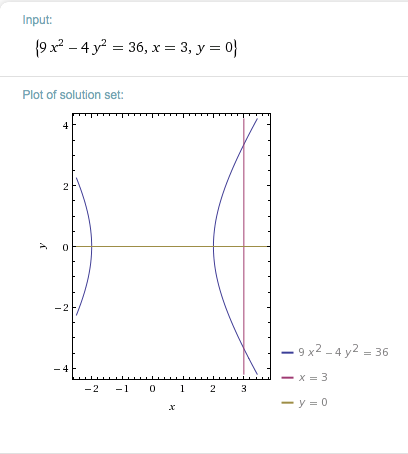
\includegraphics[width=.70\textwidth]{prob4_plot.png}\\~\\~\\~\\
The area bounded by the vertical line $x=3$ and $9x^2 - 4y^2 = 36$ is given by finding x when $y = 0$ and $x=3$.\\
When $y=0$ then $9x^2 - 4y^2 = 36$ becomes $9x^2 = 36$. \\
Thus $x = \sqrt(36/9) = 6/3 = 2$\\
Therefore we must solve the integral bounded by x = 2 and x = 3 with respect to x.\\~\\
We find the integrand by isolating the y-variable.\\
$9x^2 - 4y^2 = 36$ becomes $y = \sqrt{\frac{9}{4}x^2 - \frac{36}{4}^2}$\\
Also, because we are seeking to find the area bounded by the hyperbola and the vertical line, we must account for the portions of the function above and below the x axis.\\
Thus, we multiply the integral with respect to the positive root of the hyperbola function by two since the function is symmetric across the x-axis.\\~\\

\noindent $2 \int_2^3 \sqrt{(\frac{3}{2}x)^2-(3)^2}$\\
Because the integrand contains the form $\sqrt{u^2 - a^2}$ we use trigonometric substitution.\\
Thus, I set the "u" component, or $\frac{3}{2}x$, equal to $asec{\theta} = 3sec{\theta}$\\
Which means that $x = 2sec\theta$, and thus $dx = 2sec\theta tan\theta$.\\
We now see that the equation under the radicand becomes $(3sec\theta)^2 - 3^2$, which simplifies to $9tan^2\theta$.\\~\\
The new bounds under the u-substitution are now:\\
Upper limit, $ulim = sec^-1(\frac{3}{2})$\\ 
Lower limit, $llim = sec^-1(\frac{2}{2}) = 0$\\
For simplicity, we will indicate $sec^-1(\frac{3}{2})$ by s until the end when we evaluate the definite integral.\\~\\
$2\int_0^s \sqrt{9tan^2\theta} \left.2sec\theta tan\theta \right. d\theta$.\\
$2\int_0^s 3tan\theta 2sec\theta tan\theta d\theta$\\
$12\int_0^s sec\theta tan^2\theta d\theta$\\
$=12 \int_0^s sec\theta - sec^3\theta d\theta$\\
$=12 \int_0^s sec\theta d\theta - 12 \int_0^s sec^3\theta d\theta$\\~\\

\noindent First we evaluate $\int_0^s sec\theta d\theta$\\
We multiply the whole integral by $\frac{tan\theta + sec\theta}{tan\theta + sec\theta}$ to get $\frac{sec^2\theta + sec\theta tan\theta}{tan\theta + sec\theta}$\\
Then we use u substitution to set $u = tan\theta + sec \theta$ and thus $du = sec^2\theta + sec\theta tan\theta d\theta$\\
We then must alter the bounds.\\
The lower bound $ = tan(0) + sec(0) = 1$ and the upper bound = $tan(s) + sec(s)$, where $s = sec^{-1}(\frac{3}{2})$.\\
Therefore the upper bound $= tan(sec^{-1}(\frac{3}{2})) + sec(sec^{-1}(\frac{3}{2}))$\\
$tan(sec^-1(x)) = \sqrt{1 - \frac{1}{x^2}}x$\\
Thus the upper bound $=\sqrt{1 - \frac{1}{(\frac{3}{2})^2}}\frac{3}{2} + \frac{3}{2}$\\
This simplifies to $\frac{3}{2} + \frac{\sqrt{5}}{2}$, which we set equal to $s'$.\\
Therefore the integral is now $\int_1^{s'} u^{-1} du$, which equals $ln|u| + C$\\
$= ln|tan\theta + sec\theta|$ evaluated at lower bound 1 and upper bound s'.\\~\\

\noindent Now we consider $\int_0^s sec^3\theta d\theta$\\
$= \int_0^s \sec^2\theta sec\theta d\theta$\\
Because this is a product, we use integration by parts.\\
I set $u = sec\theta$ and thus $du = sec\theta tan\theta d\theta$.\\
I set $dv = sec^2\theta d\theta$ and thus $v = tan\theta$\\
Therefore the upper bound $sec(sec^{-1}(\frac{3}{2})) = \frac{3}{2}$ and the lower bound $=sec(0) = 1$\\

\noindent Therefore $\int_1^\frac{3}{2} sec^3\theta d\theta = tan\theta sec\theta - \int_1^{\frac{3}{2}} tan^2\theta sec\theta d\theta$.\\
We use the Pythagorean trigonometric identity to substitute $sec^2\theta - 1$ for $tan^2\theta$.\\
Thus $tan\theta sec\theta - \int_1^{\frac{3}{2}} tan^2\theta sec\theta d\theta = tan\theta sec\theta - \int_1^{\frac{3}{2}} (sec^2\theta - 1) sec\theta d\theta$\\
$= tan\theta sec\theta - \int_1^{\frac{3}{2}} sec^3\theta d\theta + \int_1^{\frac{3}{2}}sec \theta d\theta$\\
By moving $\int_1^{\frac{3}{2}} sec^3\theta d\theta$ to the left hand-side, where there is a like term, and by expanding $ \int_1^{\frac{3}{2}} sec \theta d\theta$ we get:\\
$= 2 \int_1^{\frac{3}{2}} sec^3\theta d\theta = \left. tan\theta sec\theta \right|_1^{\frac{3}{2}}+ \left. ln|tan\theta + sec\theta| \right|_1^{\frac{3}{2}}$\\
$\int_0^s sec^3\theta d\theta = \int_1^{\frac{3}{2}} sec^3\theta d\theta = \left. \frac{1}{2} tan\theta sec\theta \right|_1^{\frac{3}{2}}+  \left. \frac{1}{2} ln|tan\theta + sec\theta| \right|_1^{\frac{3}{2}}$.\\~\\

\noindent Now plugging everything back into the original formula: $=12 \int_0^s sec\theta d\theta - 12 \int_0^s sec^3\theta d\theta$\\
We get $12(\left. ln|tan\theta + sec\theta| \right|_0^{s'}) - 12(\left. \frac{1}{2} tan\theta sec\theta \right|_1^{\frac{3}{2}}+  \left. \frac{1}{2} ln|tan\theta + sec\theta| \right|_1^{\frac{3}{2}})$\\
Recall $s' = \frac{3}{2} + \frac{\sqrt{5}}{2}$\\
Therefore this definite integral equals: \\
$= 12(ln|tan(\frac{3}{2} + \frac{\sqrt5}{2}) + sec(\frac{3}{2} + \frac{\sqrt 5}{2}) - ln|tan(0)+sec(0)|) - 12(\frac{1}{2}(tan(\frac{3}{2})sec(\frac{3}{2}) - tan(1)sec(1)) + \frac{1}{2}ln| tan(\frac{3}{2}) + sec(\frac{3}{2})| - \frac{1}{2}ln|tan(1)sec(1)|$\\~\\

\noindent**I can't really evaluate any further. I checked my answer with the Wolfram calculation, and it seems that my process was the same up until the usage of some obscure "reduction" formula for the integral of $sec^3\theta$. Feedback on this would be appreciated!

\end{document}  